\chapter{Asking Las Vegas Millionaires How They Got Rich!}

This School of Hard Knocks interview, curated by LazyingArt LLC, is organized as a field search rather than a classroom lecture, but it still has a definite mathematical spine. We begin by hearing consequences before causes, then reset the city statistically, and only after that do we move through three different operator logics: commercial real estate, apparel manufacturing, and a late case about exits, catastrophic loss, banking spreads, and commercial scale. No validated board frame survives from this lecture, so the mathematics below is transcript-led and intentionally cautious.

\section{Cold Open and the Las Vegas Field}

The lecture opens by spending later outcomes before it explains where they came from. We are given loss, gain, and sale figures in quick succession:
\begin{equation}
L_{\text{Texas claim}} \approx \$30\,\text{million},\qquad
I_{\text{deal}} = \$6\,\text{million},\qquad
\Pi_{\text{deal}} \approx \$40\,\text{million},\qquad
S_{\text{sale}} = \$600\,\text{million}.
\end{equation}
At this stage these are not yet arguments. They are promises. The lecture wants us to feel scale, conflict, and risk before it tells us who these people are or how Las Vegas enters the picture.

Only after this teaser splice does the host stabilize the frame:
\begin{equation}
N_{\text{millionaires}} \approx 60{,}000,\qquad
N_{\text{billionaires}} > 10.
\end{equation}
These city counts do not function as a theorem to be proved. They function as a justification for method. If Las Vegas has this density of wealth, then moving through casinos, hotels, and restaurants becomes, in the lecture's own logic, a way of sampling commercial doctrine in the wild.

The host then narrows the field further by walking us to Bellagio. The lecture now has a location, a search rule, and a set of unresolved teaser numbers waiting to be assigned to real cases.

\section{Bellagio: Starting Small, Then Reading the Seller}

At Bellagio we first receive a short false start. A Lamborghini owner refuses the whole ``have you ever been broke'' setup and offers only a picture of his car. The lecture moves on immediately. This is worth preserving, because it tells us that luxury display is not yet the same thing as usable doctrine.

The first real operator is an older investor in shopping centers. He says he has been in real estate for
\begin{equation}
T_{\text{real estate}} = 35\ \text{years},
\end{equation}
and, when pressed on current scale, gives two concrete acquisitions:
\begin{equation}
P_{\text{Flamingo}} = \$25\,\text{million},\qquad
P_{\text{north side}} \approx \$20\,\text{million}.
\end{equation}
The order matters. He does not begin by saying ``think big.'' He begins by saying that he started small. He bought houses, and then kept building upward. Only after that ladder has been established do the shopping-center figures make sense.

The lecture then sharpens from duration and current holdings to one explicit payoff example:
\begin{equation}
I_{\text{deal}} = \$6\,\text{million},\qquad
\Pi_{\text{deal}} \approx \$40\,\text{million}.
\end{equation}
If we read the phrase ``made like \$40 million on a \$6 million investment'' at face value as profit on deployed capital, then the simplest reconstructed multiple is
\begin{align}
M_{\Pi/I}
&\approx \frac{\Pi_{\text{deal}}}{I_{\text{deal}}}
= \frac{40}{6}
\approx 6.7,\\
\text{ROI}
&\approx 667\%.
\end{align}
This is, of course, our notation rather than the speaker's, and it should remain cautious. But it captures the scale of the example he wants to put before us.

Now the lecture makes its first real conceptual turn. The operator says that every time someone is selling something, he is getting rid of a problem. The buyer's work is therefore not merely to acquire the asset, but to identify the embedded difficulty and design the exit:
\begin{equation}
\text{seller} \;\Rightarrow\; \text{problem exists},\qquad
\text{buyer} \;\Rightarrow\; \text{identify problem} + \text{design exit}.
\end{equation}
Since no literal board image survives from this lecture, we may summarize that buying logic by a small transcript-derived schematic.

\begin{figure}[h]
\centering
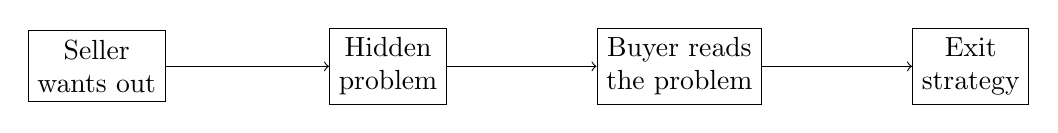
\begin{tikzpicture}
\node[draw, align=center] (a) at (0,0) {Seller\\wants out};
\node[draw, align=center] (b) at (3.7,0) {Hidden\\problem};
\node[draw, align=center] (c) at (7.4,0) {Buyer reads\\the problem};
\node[draw, align=center] (d) at (11.1,0) {Exit\\strategy};
\draw[->] (a) -- (b);
\draw[->] (b) -- (c);
\draw[->] (c) -- (d);
\end{tikzpicture}
\caption{A transcript-derived schematic of the first investor's rule: the buyer profits not merely by purchasing, but by diagnosing the seller's problem and planning the exit.}
\end{figure}

\subsection{Question \& Answer}

\paragraph{Question.} Why can a larger commercial deal be easier rather than harder?

\paragraph{Answer.} Within this operator's frame, size changes the quality of the environment. Larger deals may take longer, but they bring in more professional counterparties, cleaner financing channels, and more competent teams. The lecture does not claim that all large deals are easy. It claims something narrower and more interesting: once we cross into a different commercial tier, the structure of the game changes. Difficulty no longer grows in direct proportion to nominal deal size.

\section{Banks, Age, and the ``Different Game''}

Having moved from houses to shopping centers, and from shopping centers to seller-problem logic, the lecture now pivots into institutional asymmetry. Asked what banks do not want people to know, the first investor answers not with interest rates, but with disclosure strategy:
\begin{equation}
\text{operator rule:}\qquad \text{do not tell the bank everything}.
\end{equation}
This is a verbal equation, if one likes. The idea is that the bank wants maximal information because it wants maximal claim if trouble arises. The operator therefore treats financing as a negotiation over information, not as a neutral administrative process.

Only after that does the lecture turn to age:
\begin{equation}
a_{\text{older}} = 67,\qquad
a_{\text{host}} = 22,\qquad
\Delta a = 45.
\end{equation}
The age difference then becomes a staging ground for a dispute about work. Whose generation works harder? The older operator answers immediately: his own. The host resists. The investor answers by returning not to abstraction, but to a concrete picture of himself at twenty-two with two jewelry stores, hustling on the street, wholesaling, retailing, and traveling to Italy to buy inventory on a shoestring.

This matters because the first interview is now complete. It has given us an ascent path, a scale example, a theory of seller problems, a theory of bank asymmetry, and finally a theory of work ethic. The host then compresses all of this into a sharper doctrine:
\begin{equation}
\text{deal size} \uparrow \quad \Rightarrow \quad \text{difficulty} \downarrow
\end{equation}
within the special frame of commercial real estate, where smarter participants and easier financing offset the larger nominal scale. We should keep this speaker-framed. It is an operator's rule, not a universal law.

\section{Apparel, Brand, and the Arithmetic of Margin}

The next major case leaves property and enters apparel. Here again the order is important. The entrepreneur first gives us horizon and seriousness:
\begin{equation}
T_{\text{apparel}} \approx 10\ \text{years},\qquad
Y_{\text{apparel}} \in \text{seven figures}.
\end{equation}
But before we get to cost and price, we are given something else: this is a long-term brand. The entrepreneur is not trying to be a trend; he invokes Jay-Z and Ralph Lauren to mark the difference between flash and duration. Only after that does he turn toward unit economics.

His cleanest mathematical claim is that one must know exactly what one is manufacturing and what one is going to sell it for. The note-writer's compact form is
\begin{equation}
m = p - c,
\end{equation}
where \(p\) is selling price, \(c\) is unit production cost, and \(m\) is margin. This is not written on a board in the lecture; it is simply the most economical way to preserve the logic of what he says.

The transcript then introduces a second, more delicate margin claim. The entrepreneur speaks of overseas manufacturing, but also of local manufacturing, screen printing, and owned production steps. The safest directional reconstruction is
\begin{equation}
c_{\text{printer-owned}} < c_{\text{outsourced}}
\quad \Rightarrow \quad
m_{\text{printer-owned}} > m_{\text{outsourced}}.
\end{equation}
We should not overstate the mechanism here, because the transcript is operationally messy. But the lecture's conceptual point is clear: when we control more of the production chain, margins can widen.

He then turns from margin to community. Nike, Nordstrom, Macy's, and Tilly's appear not simply as customers, but as markers of a business level not previously reached in his specific Samoan and Polynesian context. The lecture is widening from arithmetic to social structure.

Only then do we get the purchase-order trap. A large order is not a pure blessing if the business lacks the working capital to execute it:
\begin{equation}
PO_{\text{Nordstrom}} \approx 100\ \text{racks},\qquad
K_{\text{required}} \approx 50\ \text{racks}.
\end{equation}
If we take the slang in its ordinary sense, this would mean
\begin{equation}
PO_{\text{Nordstrom}} \approx \$100{,}000,\qquad
K_{\text{required}} \approx \$50{,}000,
\end{equation}
but this dollar conversion should remain explicitly cautious. The lecture's deeper point is independent of the slang:
\begin{equation}
\text{large order} \not\Rightarrow \text{capacity to fulfill},\qquad
K_{\text{required}} > 0 \text{ before revenue arrives}.
\end{equation}

\subsection{Question \& Answer}

\paragraph{Question.} How can a large retail order become a burden instead of a breakthrough?

\paragraph{Answer.} Because an order arrives as future revenue, but fulfillment requires present structure. The entrepreneur has to finance production, labor, inventory, and timing before the money comes back. In that sense, the order is both gift and curse. It proves access, but it also tests whether the business has enough capital, relationships, and discipline to survive the very success it has just been offered.

\section{Proximity, Relationships, and Value}

After the purchase-order example, the lecture shifts again, now from working capital to motive. The apparel entrepreneur says the turning point was fatherhood and the desire to pass on generational wealth to his son. This is not a sentimental aside. It explains why the earlier arithmetic is being taken so seriously.

From there the lecture moves to proximity. He says that if the action is not in one's neighborhood, then one must go where the action is. In its cleanest conceptual form:
\begin{equation}
\text{proximity to affluent operators}
\;\Rightarrow\;
\text{relationships and opportunities}.
\end{equation}
The final phrase of that logic is spoken directly: success is about proximity.

Once the lecture arrives at this point, the closing doctrine of the apparel case follows naturally. Asked what school does not teach, the entrepreneur answers: relationships. People buy from people they like. The final maxim then tightens that into a rule about pricing:
\begin{equation}
\text{value absent} \;\Rightarrow\; \text{price becomes the issue}.
\end{equation}
This is again a speaker's commercial aphorism rather than a theorem, but it deserves to survive in note form because it compresses a large amount of selling logic into one line.

\section{Sponsor Interruption: The Side-Hustle Statistic}

The sponsor block is a true interruption and should remain one. The host says he has learned that
\begin{equation}
p_{\text{millionaires with side hustle}} = 45\%
\end{equation}
of millionaires in the United States have some kind of side hustle. The sponsor arithmetic that follows belongs to a different register:
\begin{equation}
\$10 \to \$1000,\qquad
B_{\text{bonus}} = \$50 \text{ on } \$5.
\end{equation}
These numbers should be kept structurally separate from the main entrepreneurial doctrine. They are part of the host's monetized interruption, not of the lecture's core field logic.

\section{The \$600 Million Exit, the Texas Loss, and the Last Commercial Doctrine}

The final operator resolves the largest teaser fragment. The \$600 million year came from the sale of INX:
\begin{equation}
S_{\text{INX}} = \$600\,\text{million}.
\end{equation}
This is not presented as ordinary yearly operating income. It is an exit event, and the lecture is careful to make that clear once the full case is finally opened.

Immediately after that resolution, however, the lecture reopens the earlier broke-question. The operator says he went broke because the state of Texas, with which he had a contract, refused payment, invoked sovereign immunity, and cost him
\begin{equation}
L_{\text{Texas claim}} \approx \$30\,\text{million}.
\end{equation}
We should keep this explicitly as a speaker claim. What matters for the chapter is not adjudication, but the form of the lesson that follows. His rule after catastrophic loss is not philosophical contemplation, but reset:
\begin{equation}
\text{loss} \to \text{reset next day} \to \text{new earning cycle}.
\end{equation}
He says, in effect, that one treats it like a ticket, puts it down, and starts brand new the next day.

The lecture then asks about negotiation. His answer is severe: if a prospective customer is too difficult at the front end, he would fire that customer and move on. In compact form,
\begin{equation}
\text{front-end friction too high}
\;\Rightarrow\;
\text{fire customer and move on}.
\end{equation}
The reason he gives is relational. If the relationship begins badly, it is already warning us about the rest of the contract.

\subsection{Question \& Answer}

\paragraph{Question.} When should we walk away from a customer instead of forcing the sale?

\paragraph{Answer.} In the speaker's frame, we walk away when the difficulty appears before the relationship has even properly begun. If the front end is already adversarial, then the business is being told something about the future shape of the deal. The lecture's point is not that every difficult customer must be abandoned, but that some forms of friction are predictive rather than temporary.

Asked what banks do not want people to know, the same operator gives a more quantitative answer than the earlier investor:
\begin{equation}
r_{\text{funding}} \approx 0\%,\qquad
r_{\text{customer}} \approx 10\%,\qquad
\Delta r \approx 10\%,
\end{equation}
plus fees. This is plainly rhetorical and simplified, but the institutional complaint is sharp: banks borrow cheaply, lend dearly, add fee extraction, and then use qualification standards to keep the customer cycling.

The lecture then takes one more turn, back to real estate. If one has \$100{,}000, what should one buy? He refuses the question in its residential form. He does not buy residential real estate and does not believe in residential values as his investment vehicle. He returns instead to the earlier scale doctrine: the bigger the commercial deal, the easier it can be, because the professionals, the team, and the time horizon are all there. To that he adds one more market marker:
\begin{equation}
N_{\text{empty federal buildings}} = 14{,}000.
\end{equation}
Commercial real estate, he says, is going to be an interesting market over the next twenty years.

The lecture then ends by lifting us out of business without leaving business behind. Life is not certain. Health is not certain. Relationships are not certain. Business is not certain. The only thing that is certain, he says, is God. The final image is a vertical line of orientation. In other words, the lecture's last move is to place every prior commercial technique inside a more general doctrine of instability.

\section{Summary}

This lecture proceeds by repeated conversion. It begins with consequences before causes, then resets Las Vegas as a dense field of wealth, then moves through a shopping-center investor who climbs from houses to large deals while insisting that every seller is unloading a problem, then through an apparel entrepreneur who translates brand into unit economics, margin control, working-capital stress, proximity, and relationship-based selling, and finally returns to the teaser operator whose \$600 million exit sits alongside a claimed \$30 million collapse, a next-day reset rule, a hard line on negotiation, and a hostile account of bank spreads.

What ties these segments together is not one theory of wealth, but a family resemblance among mechanisms. In one case wealth comes from reading the seller's hidden problem. In another it comes from controlling enough of production to protect margin. In a third it comes from exiting at scale and then surviving institutional predation without freezing. If we preserve that movement from anecdote, to quantity, to mechanism, then the chapter remains faithful to the lecture's actual rhythm and does not collapse into a generic summary of millionaire advice.